\pagenumbering{arabic}
\section{问题描述与背景}

蒙提霍尔问题\cite{selvin1975problem} (Monty Hall Problem) 又称三门问题、山羊汽车问题,出自美国大型游戏节目 Let's Make a Deal。

\subsection{问题描述}


现有三扇门,其中一扇门后是一辆车,另外两扇门后是一头山羊。选手从1,2,3号三扇门中选出一扇(仅标记,不打开),接着主持人再从未标记的两扇门中选出一扇打开。主持人知道每扇门后放的是什么,所以每次主持人都选择后面是羊的那扇门打开。选手有一次改变自己选择的机会。最后,打开选手最终选中的那扇门,以选手最终选择的是车为获胜。请问选手是否需要改变选择?

图 \ref{fig:Monty Hall Problem} 是一个简单易懂的图示解答。

\begin{figure}[H]
	\centering
	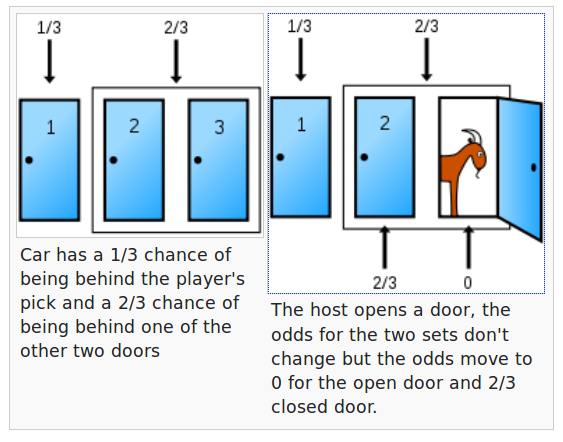
\includegraphics[width=12cm]{figure/figure1.png}
	\caption{Monty Hall Problem} \label{fig:Monty Hall Problem}
\end{figure}

\subsection{相关背景}

对于此问题,主持人 Monty Hall 认为换与不换选中汽车的概率都是 $\frac{1}{2}$;1975 年 Selvin Steve 对主持人的说法提出了质疑,并利用古典概率公式给出换门和不换门选中汽车的概率分别为 $\frac{2}{3}$ 和 $\frac{1}{3}$,由此引发了众多的争议。

争论双方都认可的的表述有:
\par{(1) 假设游戏开始前汽车被等概率地放置在每一扇门的后面;}
\par{(2) 游戏参与者初始选择是随机的,即在三扇门中随机地选定其中的一扇;}
\par{(3) 游戏参与者的选择和汽车的放置是相互独立的;}
\par{(4) 主持人对于门后奖品的分布知情,主持人不会打开游戏参与者初始选定的门,也不会打开有汽车的门,只会打开有山羊的门。}

用 $A_1,A_2,A_3$ 分别表示 $1,2,3$ 号门后面是车,$B_1,B_2,B_3$ 分别表示选手打开 $1,2,3$ 门,$C_1,C_2,C_3$ 分别表示主持人打开 $1,2,3$ 号门。有部分人给出了下面的做法,基于 $B_1C_3$ 已经发生的条件下,利用条件概率解答,由 (1) 可以确定

\begin{align}
P(A_1)=P(A_2)=P(A_3)=\frac{1}{3}
\end{align}

由 (1) 至 (3) 得

\begin{gather}
P(A_iB_j)=\frac{1}{9}, \\
P(A_i|B_j)=P(B_j|A_i)=\frac{1}{3},\quad1\le i,j\le3
\end{gather}

由 (4) 得

\begin{gather} \label{question}
P(C_2|A_1B_1)=P(C_3|A_1B_1)=\frac{1}{2}\\
P(C_3|A_2B_1)=P(C_3|A_3B_1)=0
\end{gather}

因此,游戏参与者打开 1 号门,并且主持人打开门 3 的概率为

\begin{align*}
P(B_1C_3)&=\sum_{i=1}^3P(A_iB_1C_3)\\
&=\sum_{i=1}^3P(A_i)P(B_1|A_i)P(C_3|A_iB_1)\\
&=\frac{1}{3}\times\frac{1}{3}\times(\frac{1}{2}+1+0)\\
&=\frac{1}{6}
\end{align*}

选手采用坚持策略获得汽车的概率为

\begin{align*}
P(A_1|B_1C_3)&=\frac{P(A_1B_1C_3)}{P(B_1C_3)}\\
&=6P(A_1B_1)P(C_3|A_1B_1)\\
&=6\times\frac{1}{9}\times\frac{1}{2}=\frac{1}{3}
\end{align*}

选手采用改变策略选 2 号门获得汽车的概率为

\begin{align*}
P(A_2|B_1C_3)&=\frac{P(A_2B_1C_3)}{P(B_1C_3)}\\
&=6P(A_2B_1)P(C_3|A_2B_1)\\
&=6\times\frac{1}{9}\times1=\frac{2}{3}
\end{align*}

这样就得到了与 Selvin Steve 相同的结论。有学者\cite{李勇2018三门问题}指出式 ( \ref{question} ) 实际上并不严谨,在三门问题中没有规定主持人是以等概率在选手选剩下的山羊门中选择打开的门,为了正确计算,我们添加限制如下,

\par{主持人在选手选剩下的有山羊门中以概率 $p$ 打开编号最大的门。}

按照之前解法的思路我们可以得到

\begin{align*}
P(B_1C_3)&=\sum_{i=1}^3P(A_iB_1C_3)\\
&=\sum_{i=1}^3P(A_i)P(B_1|A_i)P(C_3|A_iB_1)\\
&=\frac{1}{3}\times\frac{1}{3}\times(p+1+0)=\frac{p+1}{9}
\end{align*}

选手采用坚持策略获得汽车的概率为

\begin{align*}
P(A_1|B_1C_3)&=\frac{P(A_1B_1C_3)}{P(B_1C_3)}\\
&=\frac{9}{p+1}\times P(A_1B_1)P(C_3|A_1B_1)\\
&=\frac{9}{p+1}\times\frac{1}{9}\times p\\
&=\frac{p}{p+1}
\end{align*}

选手采用改变策略选 2 号门获得汽车的概率为

\begin{align*}
P(A_2|B_1C_3)&=\frac{P(A_2B_1C_3)}{P(B_1C_3)}\\
&=\frac{9}{p+1}\times P(A_2B_1)P(C_3|A_2B_1)\\
&=\frac{9}{p+1}\times\frac{1}{9}\times1\\
&=\frac{1}{p+1}
\end{align*}

由此该学者得出结论,对于任意 $p\in[0,1]$ 总有

$$\frac{p}{p+1}\le\frac{1}{p+1}$$

即选手换门得到汽车的概率总是大于等于坚持策略获得汽车的概率。

但实际上该学者的论证过程和上面的一个思路都是错误的,至于为什么,我们之后再进行讨论。